\documentclass{beamer}
\usepackage[export]{adjustbox}
\usepackage{tikz}
\usepackage{animate}
\usepackage[utf8]{inputenc}
\usepackage{textcomp}

\begin{document}


\begin{frame}{ARF2 and ARF5 DapSeq regions}
  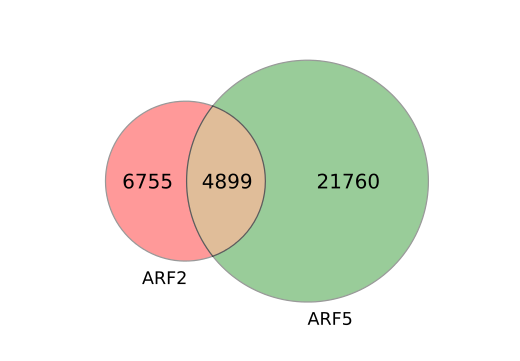
\includegraphics[width=1\textwidth,height=0.8\textheight,center]{Venn.png}
\end{frame}

\begin{frame}
\centering
\Huge{How to predict ARFs binding sites ?}
\end{frame}


\begin{frame}{ROC best score on all the regions (OMalley monomer matrices)}
  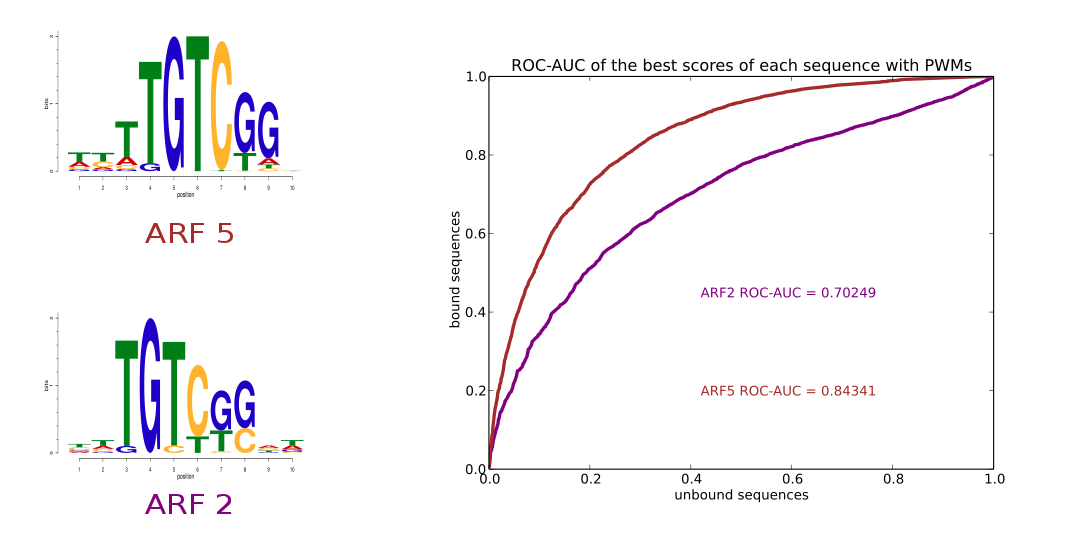
\includegraphics[width=1\textwidth,height=0.8\textheight,center]{ROC_et_logo.png}
\end{frame}


\begin{frame}{How negative sets are built for 1000 regions}
  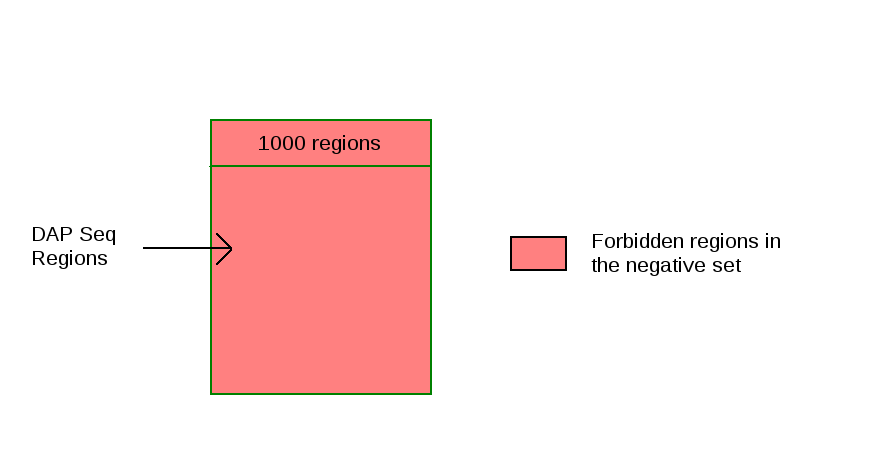
\includegraphics[width=1\textwidth,height=0.8\textheight,center]{negative_set_all_regions.png}
\end{frame}


\begin{frame}{Let suppose the 1000 first regions are the true one bound}
  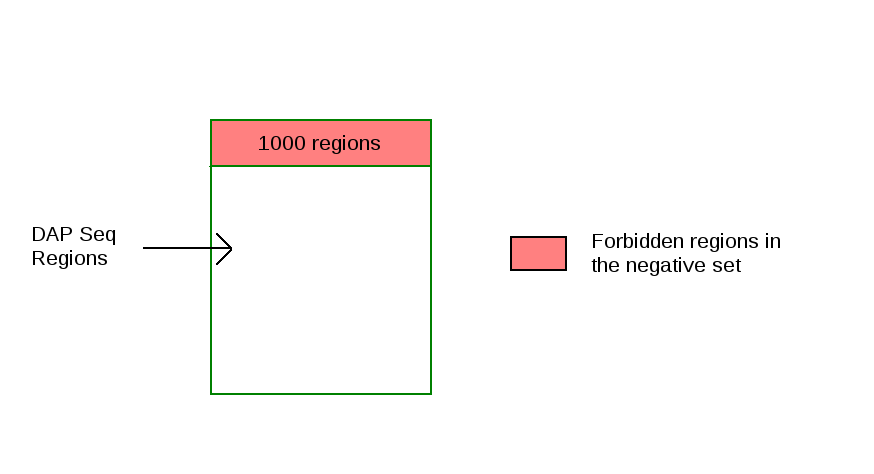
\includegraphics[width=1\textwidth,height=0.8\textheight,center]{negative_set_1000_regions.png}
\end{frame}


\begin{frame}{1000 first regions of the DAPSeq - ARF2 (first method)}
  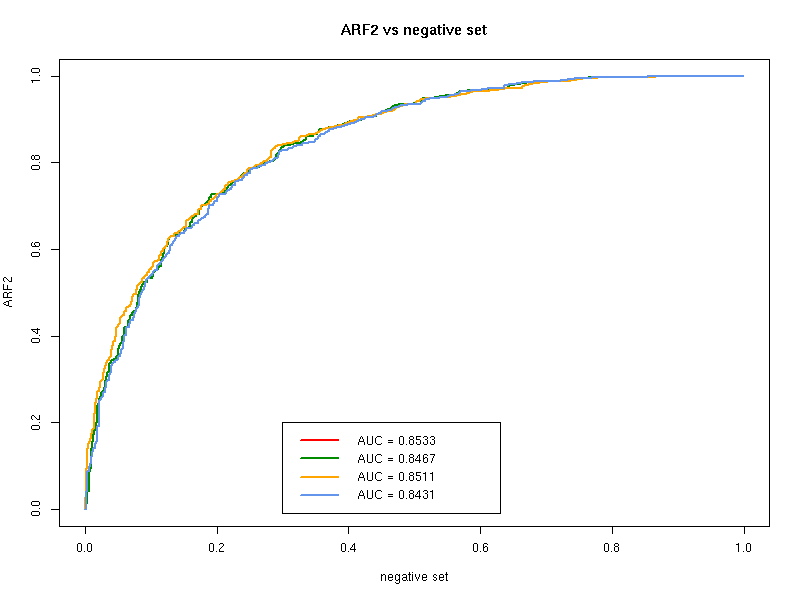
\includegraphics[width=1\textwidth,height=0.8\textheight,center]{ROC_ARF2_negative_set_all_regions.png}
\end{frame}

\begin{frame}{1000 first regions of the DAPSeq - ARF2 (second method)}
  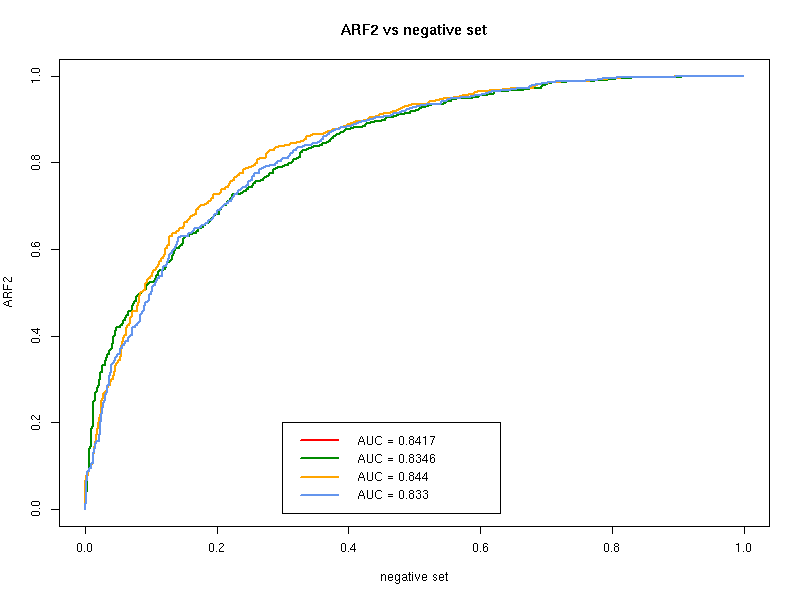
\includegraphics[width=1\textwidth,height=0.8\textheight,center]{ROC_ARF2_negative_set.png}
\end{frame}


\begin{frame}{1000 first regions of the DAPSeq - ARF5 (first method)}
  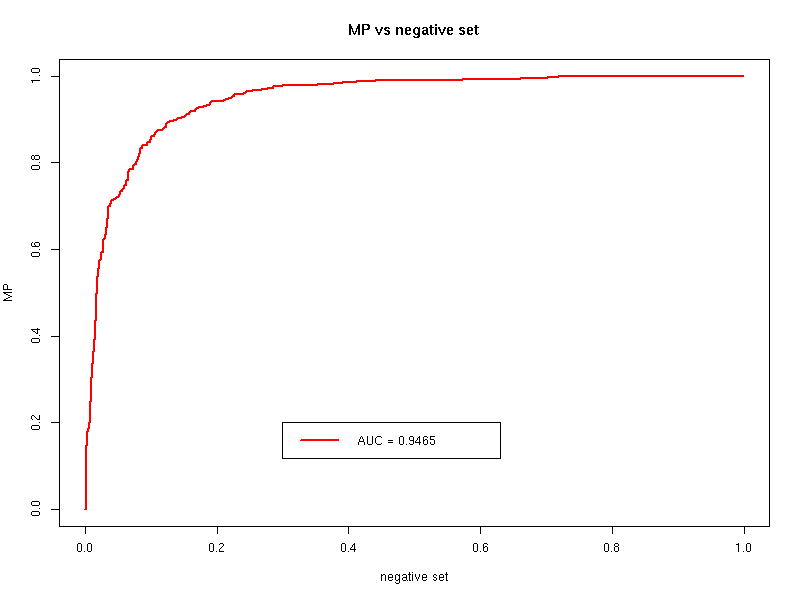
\includegraphics[width=1\textwidth,height=0.8\textheight,center]{ROC_MP_negative_set_all_regions.png}
\end{frame}


\begin{frame}{1000 first regions of the DAPSeq - ARF5 (second method)}
  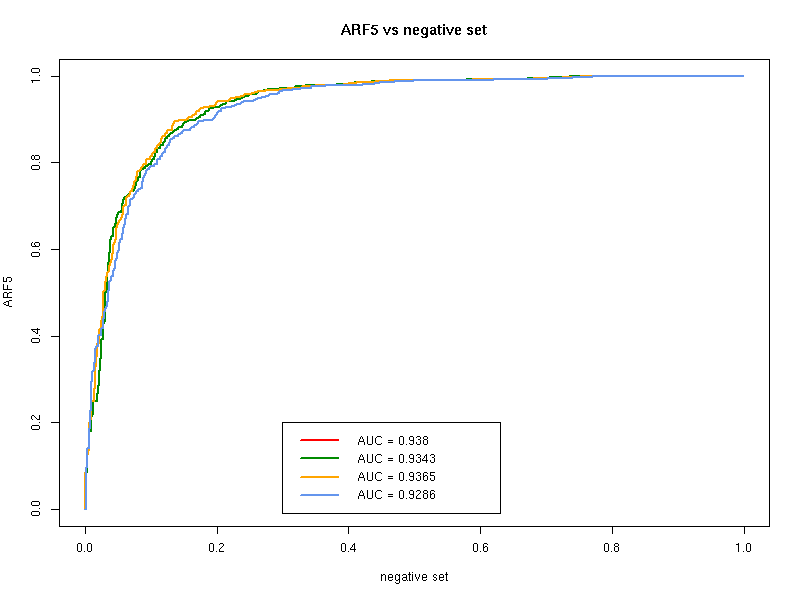
\includegraphics[width=1\textwidth,height=0.8\textheight,center]{ROC_ARF5_negative_set.png}
\end{frame}

\begin{frame}
\centering
\Huge{Predictions vs wet lab}
\end{frame}

\begin{frame}{Comparisons EMSAS DAPSeq - ARF5}
  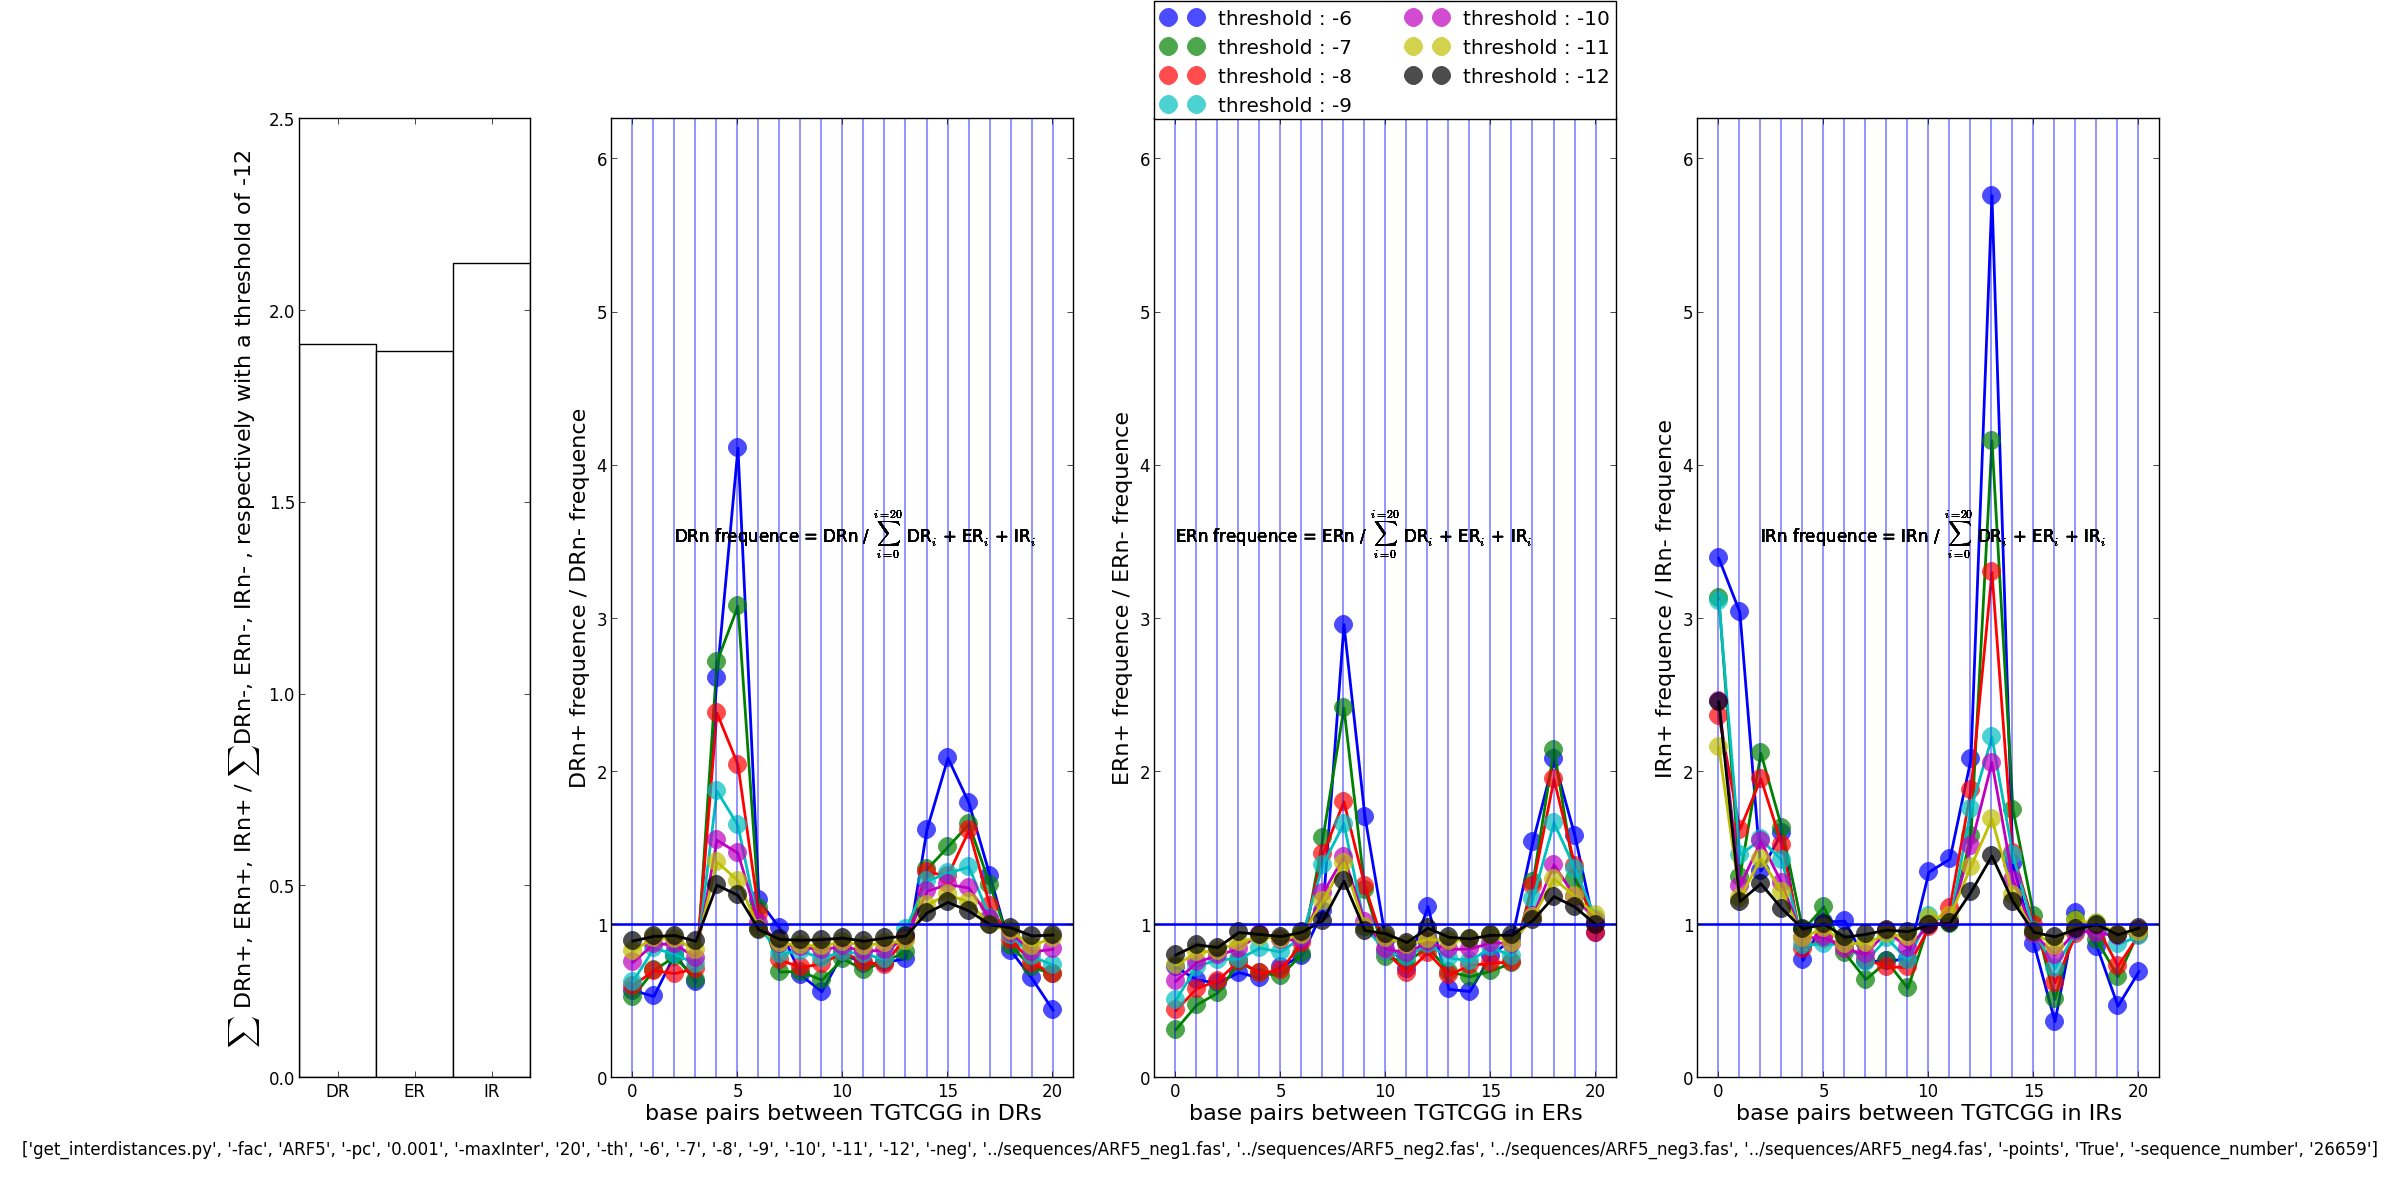
\includegraphics[width=1\textwidth,height=0.8\textheight,center]{ARF5_interdistances_-6-7-8-9-10-11-12_points_4Neg.png}
\end{frame}

\begin{frame}{Comparisons EMSAS DAPSeq - ARF2}
  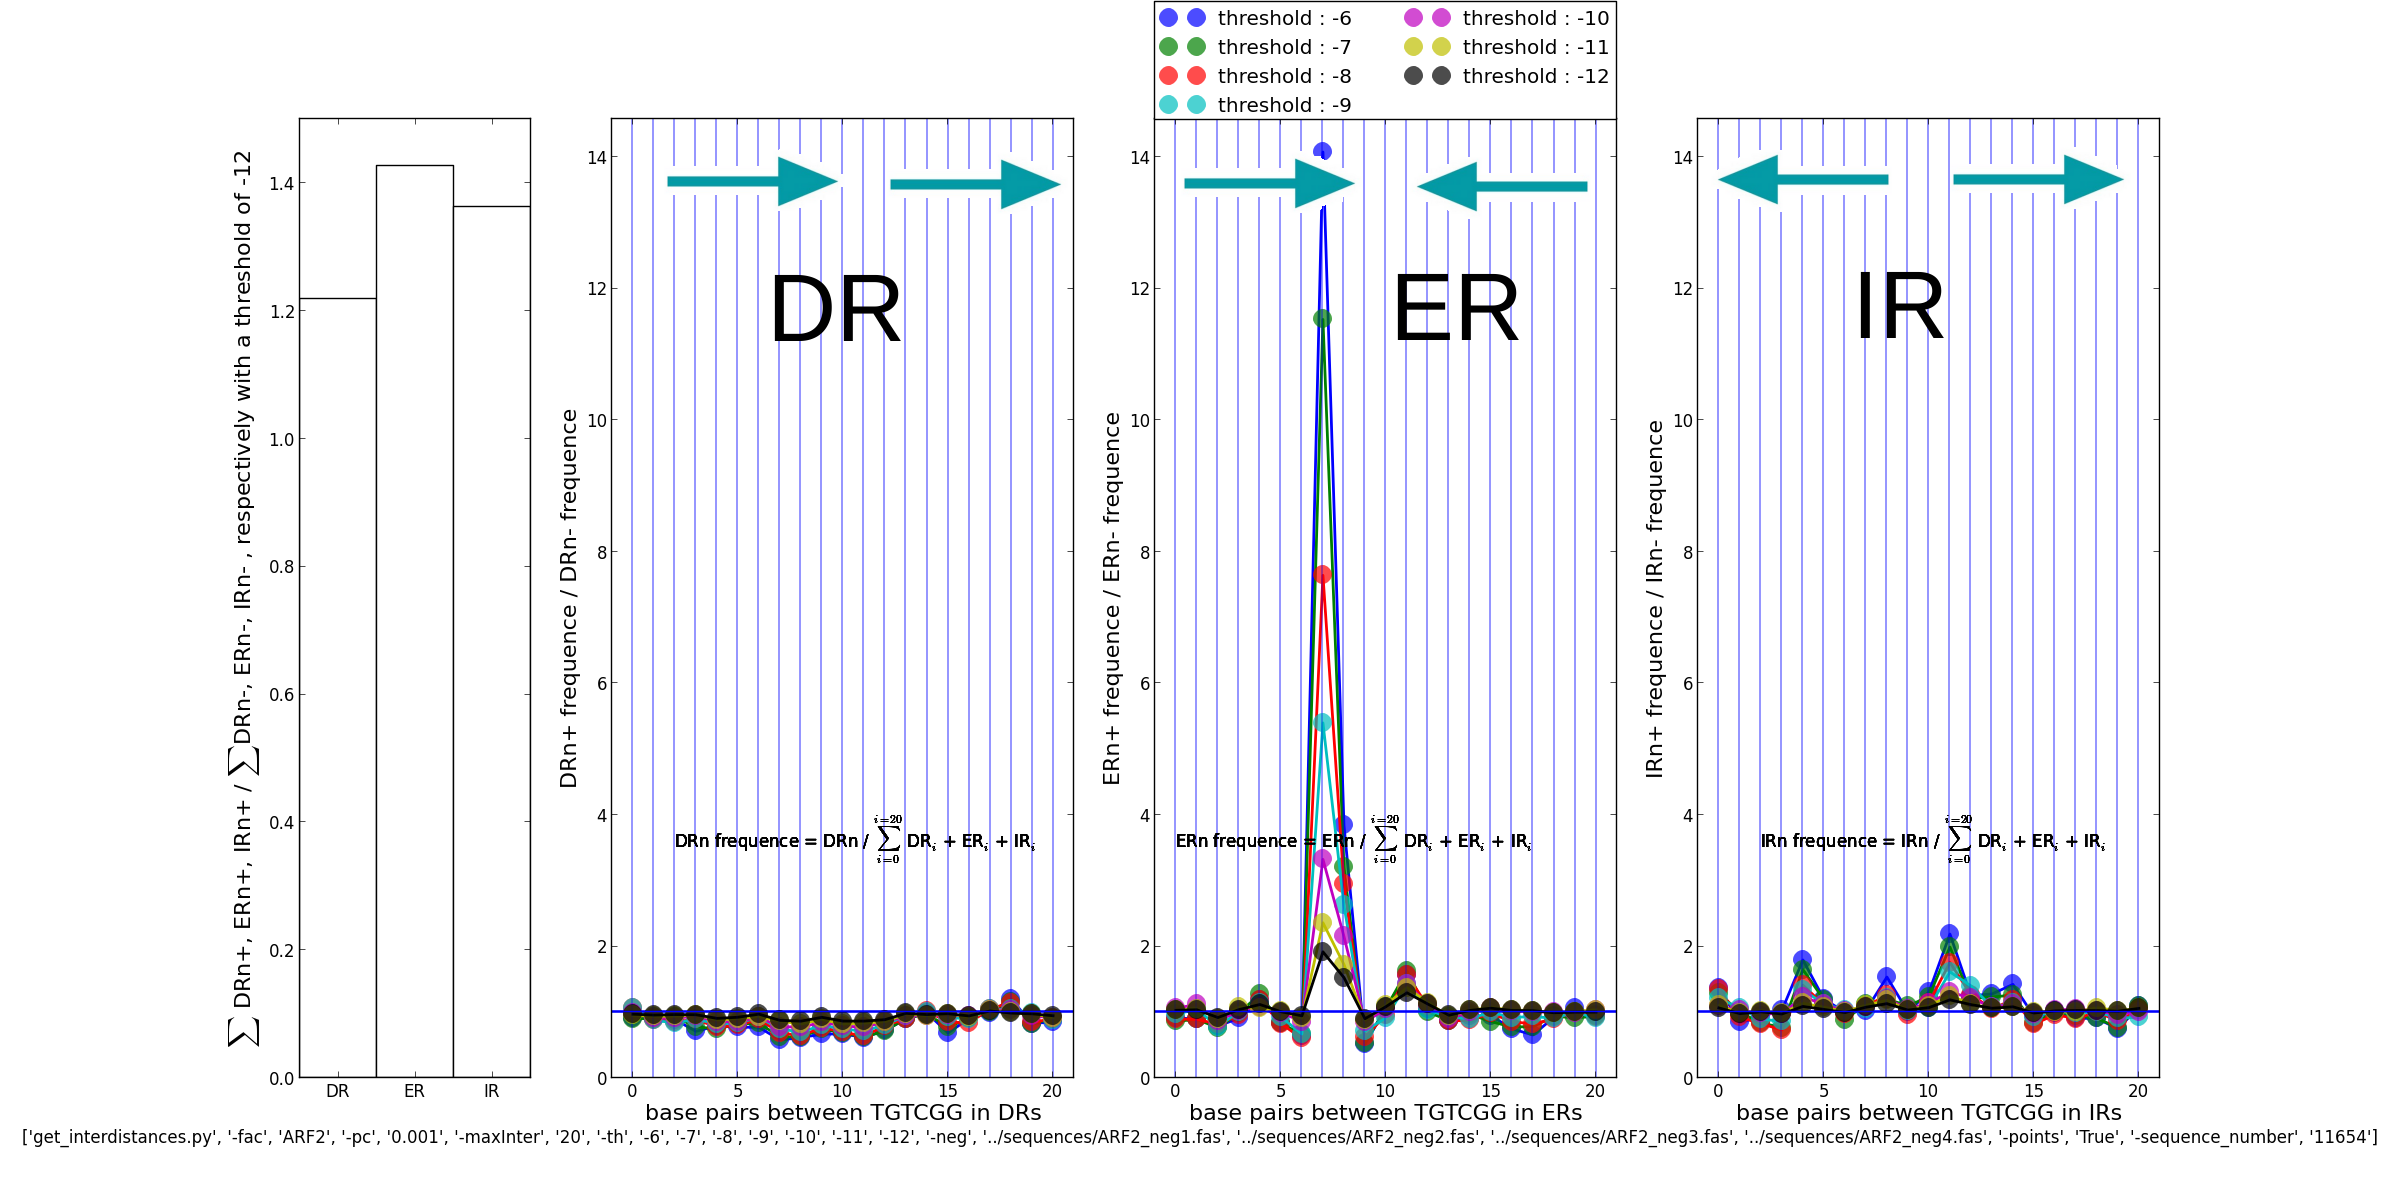
\includegraphics[width=1\textwidth,height=0.8\textheight,center]{ARF2_interdistances_-6-7-8-9-10-11-12_points_4Neg.png}
\end{frame}

\begin{frame}{Comparisons EMSAS DAPSeq - EMSAS DR}
  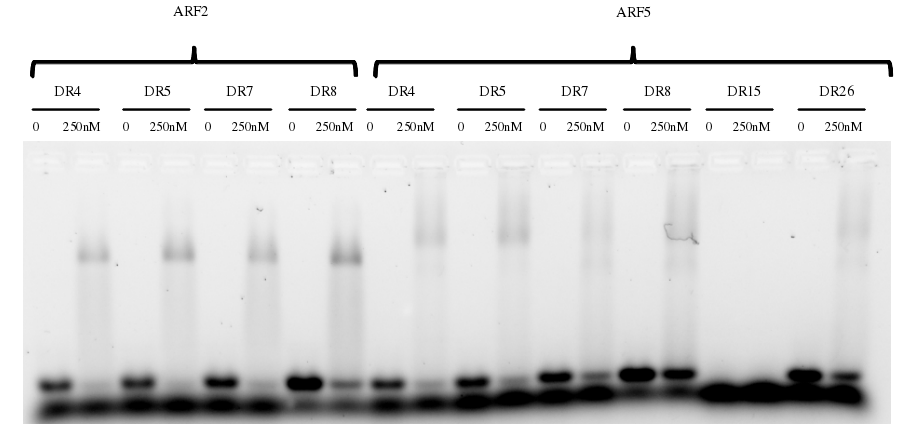
\includegraphics[width=0.9\textwidth,height=0.8\textheight,center]{EMSA_DR.png}
\end{frame}

\begin{frame}{Looking for some DNA features}
  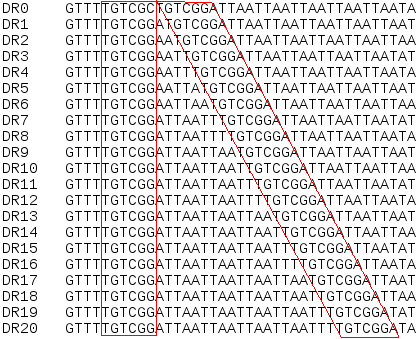
\includegraphics[width=0.77\textwidth,height=0.7\textheight,center]{tableau_DR.png}
\end{frame}

\begin{frame}{Looking for some DNA features}
  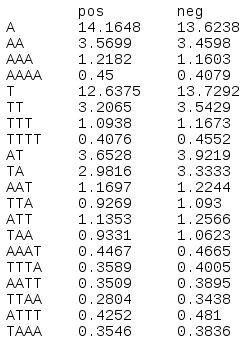
\includegraphics[width=0.5\textwidth,height=0.6\textheight,center]{A_and_T_rate.png}
\end{frame}

\begin{frame}{Methylation ?}
  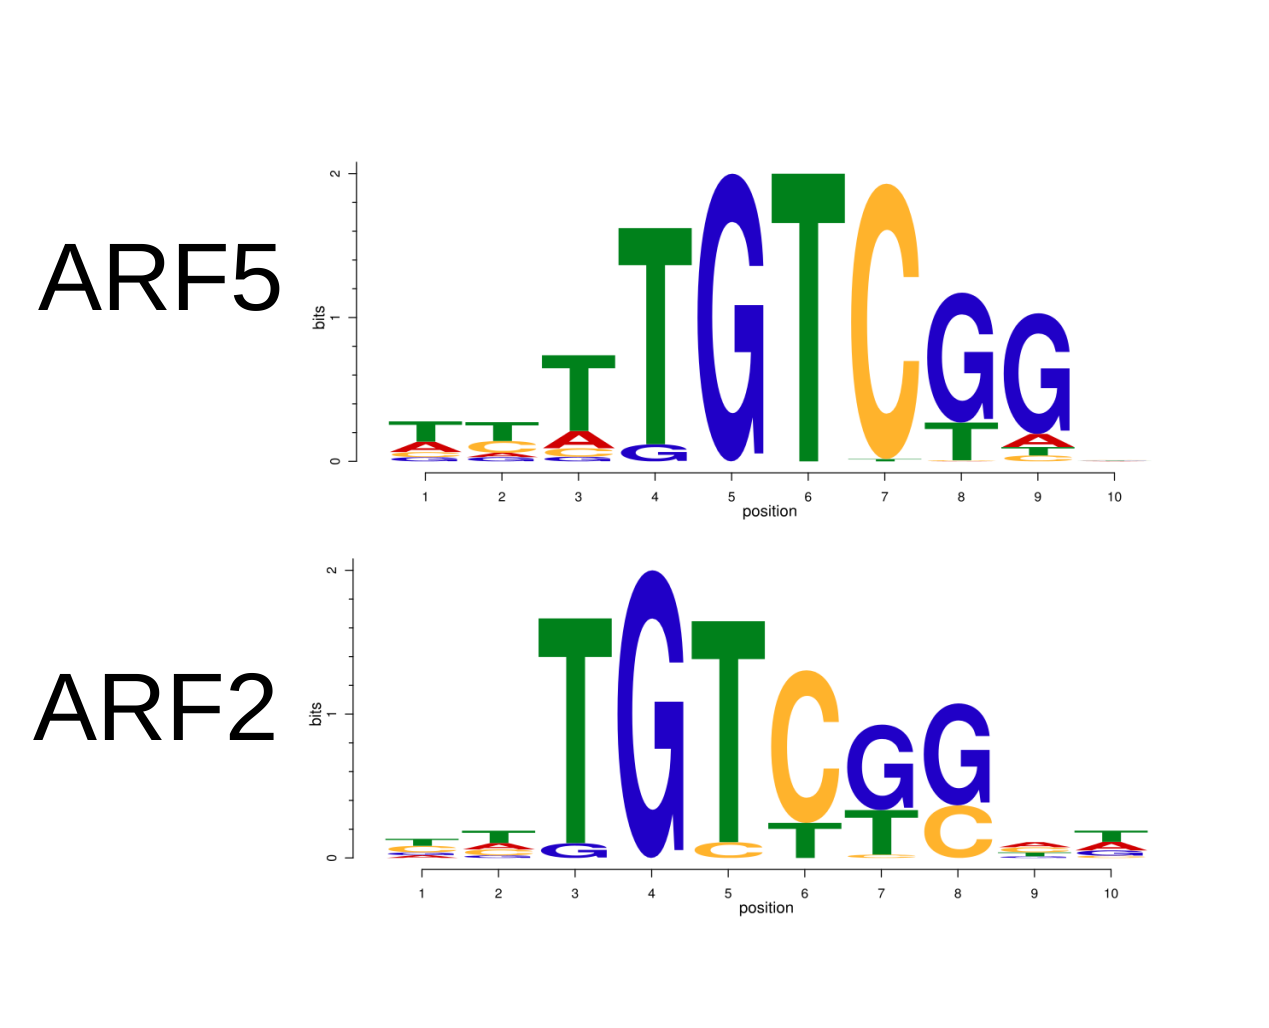
\includegraphics[width=1\textwidth,height=0.90\textheight,center]{logos.png}
\end{frame}

\begin{frame}{Methylation ?}
  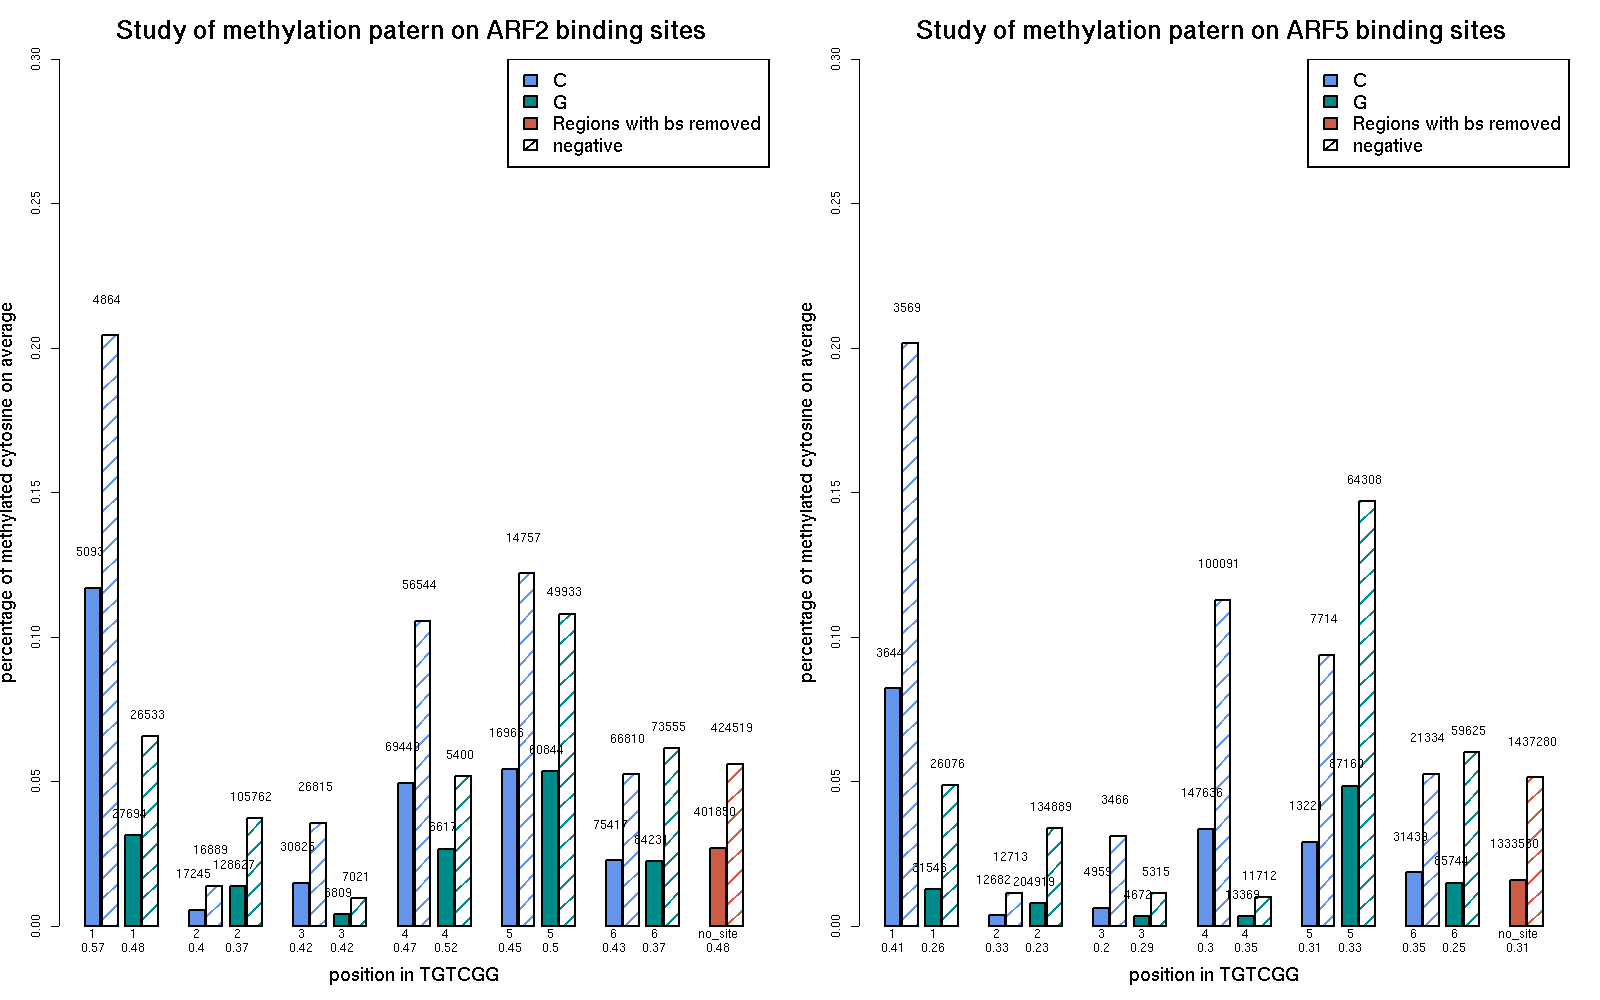
\includegraphics[width=1\textwidth,height=0.90\textheight,center]{ARF2_ARF5_methylation_and_sample_sizes_v3.png}
\end{frame}




\end{document}
%%% Local Variables:
%%% mode: latex
%%% TeX-master: t
%%% End:
